%\usepackage{graphicx}

\chapter{Implementation}\label{ch:implementation}

\section{Approach}

Our aim was to create a more personalized view of the Facebook feed. The top down approach was used to break the problem into smaller modules and to create a solution for each module. The problem was broken down into the following parts:

\begin{itemize}
	\item Pulling data from the Facebook feed
	\item Ranking Algorithm
	\item User Interface
\end{itemize}

To implement this solution we have used Nodejs for a number of reasons: 

\begin{itemize}
	\item It is a very flexible and diverse language and can be used for a huge variety of purposes, allowing us to create all aspects of our system using it.
	\item Many user-made modules that allow us to reuse solutions, e.g. interfacing with the Facebook api
	\item It is essentially just javascript which is perfect for a light application such as ours
\end{itemize}

\newpage
\section{Facebook API and App}

Facebook requires the creation of an app in order to allow a website to pull any data from a user’s account. In order to create the application we registered as Facebook developers and were given a unique App ID and secret for our application. This is used to let Facebook know that our application is being used when we make calls to Facebook's API.

To grab the feed data from Facebook we utilized the Nodejs module written by Thuzi. This module communicates with the Graph API provided by Facebook that is used to gather information from the feed. Another module that was used was the passport-facebook module written by Jared Hanson. This module was mainly used to allow ease of authentication for Facebook. This means that we do not directly control the authentication and we are not capable of storing usernames or passwords.

Before we can begin pulling data from the feed we first need to get permissions from the user about which data that we need. The permissions that we desired were:

\begin{itemize}
	\item read stream (feed)
	\item user likes
	\item read mailbox
\end{itemize}

The reason for getting each of these permissions will be explained in the ranking algorithm.

We receive the user’s feed as a json object, containing a huge amount of data on each feed item. We proceed to extract the required information and create our own feed item object, containing the fields shown in the figure 4.1, below.

\begin{center}
\includegraphics[scale=0.8]{images/UMLFeed.png}
\captionof{figure}{FeedItem UML}
\end{center}

The name is the name of the person or organisation that posted the feed item. 

The ID is the ID of the person or organisation that posted the feed item.

The category is Facebook’s generated category of the feed item.

The message is the message of the feed item that appears in text.

The picture is a url of a feed item that points to a picture. This is relevant if the type is photo.

The link is a url that points to the actual feed item.

The type is the type of the feed item. It could be a photo or video.

The action is the action that was taken on the feed item.

The source is a url of a feed item. This is only relevant if the type is a video.

The createdTime is the time the feed item was created.

\newpage
\section{Ranking Algorithm}

The algorithm for ranking the feed from Facebook comes from the combination of many other algorithms that have been specified in our design. The algorithm contains the following key components:

\begin{itemize}
	\item Topic Classification
	\item Connections
	\item Freshness
	\item Diversity
	\item User Modelling
\end{itemize}

Each set component will provide either a positive or negative score to each feed item that we have received from the feed.

\subsection{Pseudocode}

\begin{center}
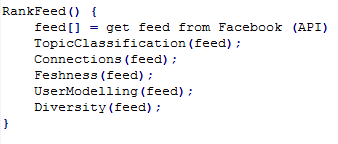
\includegraphics[scale=0.8]{images/allPseudo.png}
\captionof{figure}{Pseudocode for Ranking Algorithm}
\end{center}

\subsection{Topic Classification Module}
The Topic classification module followed an idea from Szo~\cite{szomszor2008semantic} where a search of Wikipedia can be used on tags in order to generalise the topic. We decided to go through the user's likes and to do a wikipedia search in order to determine the topic of interest. To get this data we require the read likes permission from Facebook. The Wikipedia search used a nodejs module called wikipedia-js written by kenshiro. When we get a feed item from the feed, we would check parts of the feed for a match for the topics we generalised from wikipedia. A match would mean that the topic of interest of the user has appeared in the particular feed item and hence, we would add a positive score to the feed item.

\begin{center}
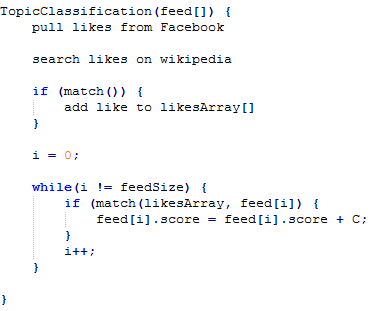
\includegraphics[scale=0.8]{images/topicClassification.png}
\captionof{figure}{Pseudocode for Topic Classification Module}
\end{center}

\subsection{Connections Module}
The Connections module was based on the idea from Li~\cite{LiTiaLee2010} where a user may prefer a feed item that their friend likes or feed items. Our implementation of this module involved looking at the friends that the user has recently messaged. This required the read mailbox permission from Facebook. We do not directly look into the message but do consider the friend that the user has recently talked to. We consider the items from the feed where the person who posted the feed item is a friend of the user. We would add a positive score to the feed item if the poster and the user are friends that have recently interacted.

\begin{center}
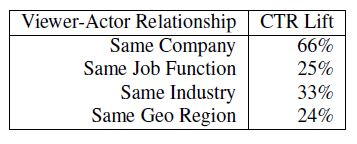
\includegraphics[scale=0.8]{images/connections.png}
\captionof{figure}{Pseudocode for Connection Module}
\end{center}

\subsection{Freshness and Diversity Module}
The Freshness module implementation followed an idea from Aga~\cite{Aga2014} where we assigned an initial score to each feed item and decreased the score depending on the feed item’s creation time. For the diversity module, we used an array to store all the types of feed items that we have not seen before. As the feed items come, we compare the feed items with the array of feed items in the array. The fields that we consider are type, category, name and link. If there is a match then we have seen a similar feed item before and should subtract score in order to make our feed more diverse. If there isn’t a match then we add it to the array.

\begin{center}
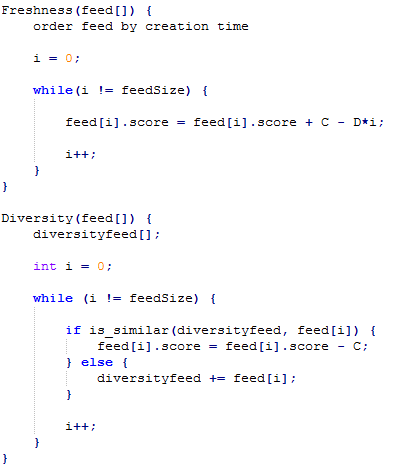
\includegraphics[scale=0.8]{images/freshDiv.png}
\captionof{figure}{Pseudocode for Freshness and Diversity Module}
\end{center}

\subsection{User Modelling}
User modelling came from Bon~\cite{bonds2010myspace} and Nad~\cite{nadkarni2012people} who concluded users have different reasons for using Facebook. This module hopes to find a generalized user and adapt the feed to their particular needs. Some types of users we generalised were:

\begin{itemize}
	\item A \textbf{Socialite} is a user who mainly uses Facebook to see feed items from friends or families.
	\item A \textbf{News Reader} is a user who mainly uses Facebook to keep up-to-date with the news.
	\item A \textbf{Follower} is a user who uses Facebook to see feed items from organisations.
\end{itemize}

These user types were created based on intuition, which is why we carried out the survey specified in the design section. We created our survey using an online survey tool called SurveyMonkey. This allowed us to input our questions (as seen in figure 3.1) into an online platform to share with participants.

To distribute our surveys in a way that the participants would be diverse and unbiased, we made use of SurveyMonkey’s feature of purchasing responses. This process works as follows; when a participant completes a survey with SurveyMonkey, they are (at random) asked whether they would like to join their panel, which would involve being invited to complete surveys where the profits from the purchased responses go towards charity. This creates an organic, unbiased panel of participants ready to give responses to surveys.

We chose to make our survey available to participants in the US of all ages, ethnicities and gender, with the only restriction being that they must be Facebook users, of course.
We received over 100 responses which we analysed for any notable patterns. The responses were of surprisingly good quality and quite diverse and in depth. Some interesting points we observed were:

\begin{itemize}
\item Some users suggested we consider more specific post types such as weather alerts, free giveaways and local stories, while this would be great, given our time constraint it would be impractical for us to implement.
\item A significant amount (~10 percent) of users provided quite a surprising response in regards to connections, that was that they would prefer to see content from friends who they did not interact with often. These types of users could be accommodated for in our system as a subtype of socialite, however we did not increase the number of user types as we wanted to keep it general and lessen how much the user had to think about their user type. This decision was made after seeing how difficult it was for users to determine their own user types even with our 3 basic, generalised types. This is further discussed in the evaluation section. 
\end{itemize}

The raw data can be seen in Figure 4.6

\begin{center}
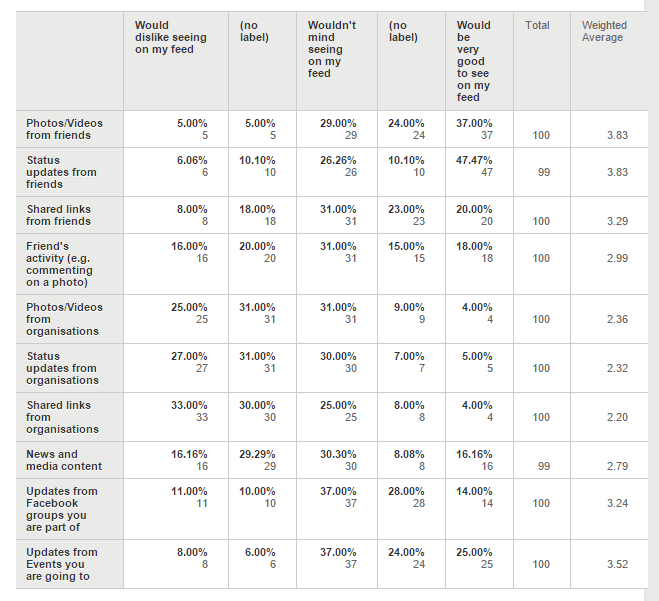
\includegraphics[scale=0.8]{images/surveyTable.png}
\captionof{figure}{Table of users}
\end{center}

These results only indicate the opinions of the sample in general, to observe for patterns in user types, we had to analyse each response individually, categorise them as either Socialite, Follower, News Reader, or none. This process yielded the following graph:

\begin{center}
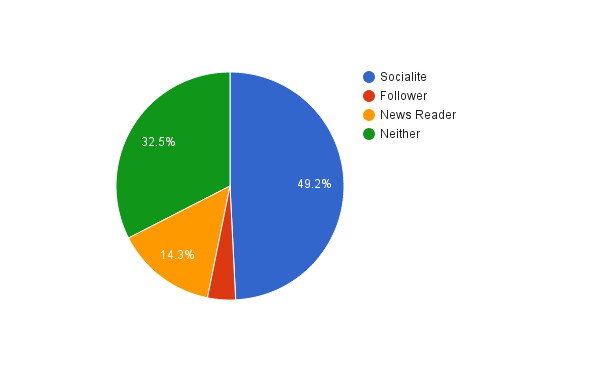
\includegraphics[scale=0.8]{images/usermodelChart2.png}
\captionof{figure}{Pie chart of user type distribution}
\end{center}

One could argue that the follower type may not be a significant portion of the results, however we struggled to find any other significant pattern of users from our survey responses and the follower type definitely did stand out to us. From this analysis, we were quite confident in using the aforementioned user types for the user modelling component of our algorithm.

The weightings for each of these user types are explained as follows:
\begin{itemize}
\item Users who identified as socialites had additional score added to their feed items if the feed item was generated by the action of a friend (e.g. ‘liked’ the feed item) and even more score was added if the feed item was actually posted by the friend.
\item Users who identified as News readers had additional score added to their feed items if the category field contained “news” in the string. This created some problems with the diversity algorithm as the score would then be subtracted due to feed items having the same category, so we bypassed that section of the diversity module if the user identified as a news reader.
\item Users who identified as Followers acted oppositely to a socialite, that is, we added additional score to the feed item if it was generated by the action of an entity who is not a friend and additional points if it was posted by that entity themselves.
\end{itemize}

\begin{center}
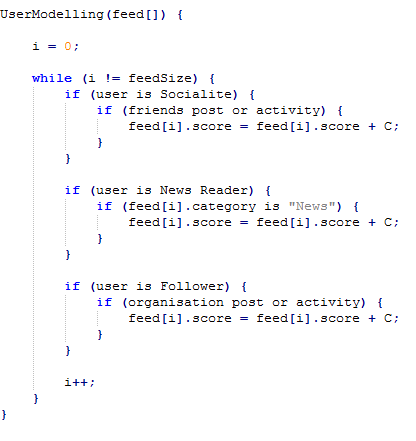
\includegraphics[scale=0.8]{images/userModel.png}
\captionof{figure}{Pseudocode for User Modelling Module}
\end{center}

\newpage
\section{User Interface}

A typical user that uses our app will first be welcomed with a welcome screen as shown in the figure below.

\begin{center}
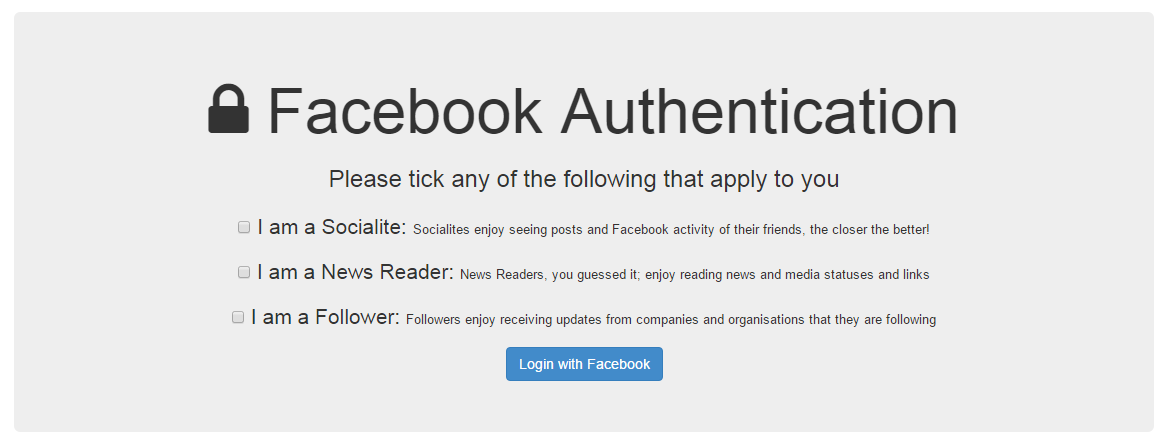
\includegraphics[scale=0.5]{images/mainscreen.png}
\captionof{figure}{Welcome screen}
\end{center}

The user can choose one or more of the options before they click log in. When the login is clicked, the user is taken to a typical login screen from Facebook.

After logging in, the user will be able to see a Facebook feed.

\begin{center}
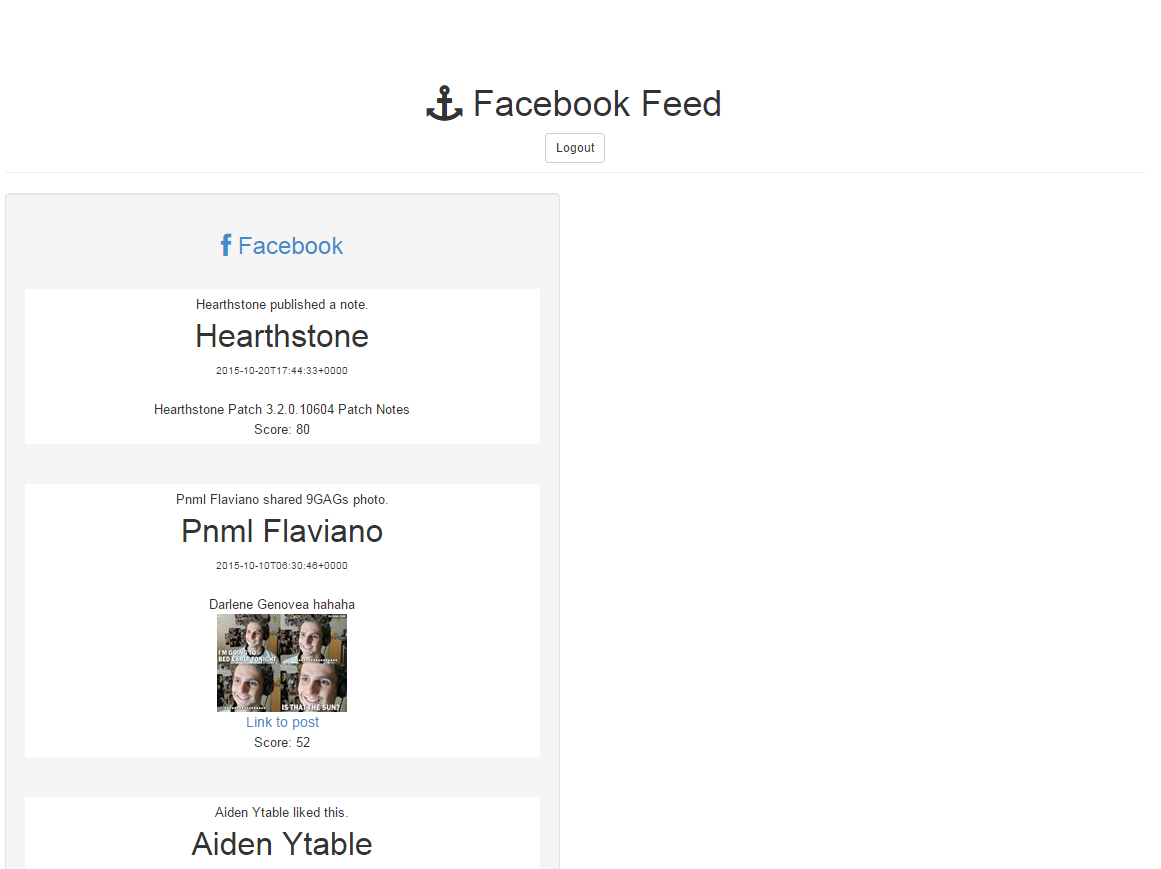
\includegraphics[scale=0.5]{images/rankedFeed.png}
\captionof{figure}{Profile Page with ranked feed}
\end{center}

\newpage
\section{Problems Encountered}

A typical user receives an enormous amount of items to their feed daily. This means that we would be required to pull a large amount of feed items in order to decide which items that the user would prefer to see. Unfortunately Facebook has a limitation on how many API calls can be made in a period of time. Only 600 API calls can be made every 10 minutes. This limitation has prevented us from getting more data about the user such as searching through the feed to see if a friend has liked a particular feed item.

Additionally it may seem that some of our modules such as the connections module seem far too simple. This was also due to restrictions placed on us by the Facebook API; one such limitation of the Facebook API involved the friends list. The Facebook API only allows us to get friends who have also installed the app. For our particular time frame, this is very impractical, thus we were unable to even see a list of the user's friends, let alone data about how close they are.

Another limitation that we encountered was not having access to the user’s own past posts, this meant that we had to resort to only looking at the user’s ‘liked’ pages to define their topics of interest, instead of looking at their past posts as suggested by Szo~\cite{szomszor2008semantic}.